\documentclass[tikz,border=10pt]{standalone}
\usepackage{tikz}
\usetikzlibrary{positioning,arrows.meta,shapes,calc,patterns}

\begin{document}
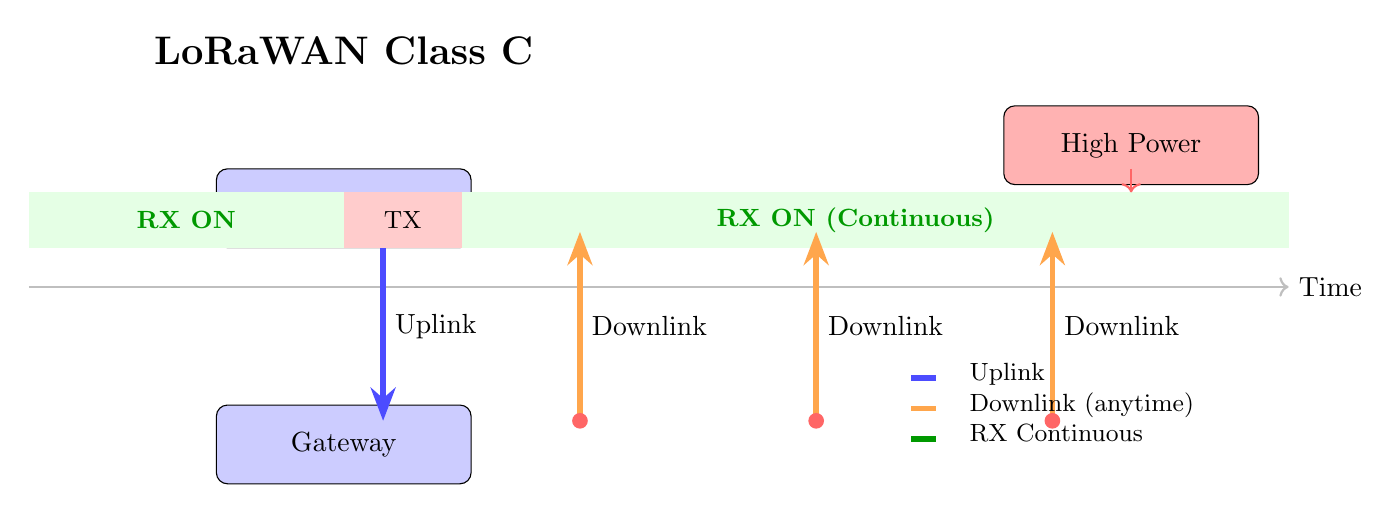
\begin{tikzpicture}[
    node distance=1.5cm,
    block/.style={rectangle, draw, fill=blue!20, text width=3cm, text centered, rounded corners, minimum height=1cm},
    arrow/.style={-Stealth, thick},
    timeline/.style={->, thick, draw=gray!50},
    event/.style={circle, fill=red!60, inner sep=2pt}
]

% Title
\node[font=\Large\bfseries] at (0,5) {LoRaWAN Class C};

% Device
\node[block] (device) at (0,3) {End Device};

% Gateway
\node[block] (gateway) at (0,0) {Gateway};

% Timeline
\draw[timeline] (-4,2) -- (12,2) node[right] {Time};

% Continuous RX (shaded area)
\fill[green!10] (-4,2.5) rectangle (0,3.2);
\fill[green!10] (1.5,2.5) rectangle (12,3.2);
\node[font=\small\bfseries, green!60!black] at (-2,2.85) {RX ON};
\node[font=\small\bfseries, green!60!black] at (6.5,2.85) {RX ON (Continuous)};

% Uplink
\draw[arrow, blue!70, line width=2pt] (0.5,2.7) -- node[right, black] {Uplink} (0.5,0.3);
\node[event] at (0.5,2.7) {};
\fill[red!20] (0,2.5) rectangle (1.5,3.2);
\node[font=\small] at (0.75,2.85) {TX};

% Downlink can happen anytime
\draw[arrow, orange!70, line width=2pt] (3,0.3) -- node[right, black] {Downlink} (3,2.7);
\node[event] at (3,0.3) {};

\draw[arrow, orange!70, line width=2pt] (6,0.3) -- node[right, black] {Downlink} (6,2.7);
\node[event] at (6,0.3) {};

\draw[arrow, orange!70, line width=2pt] (9,0.3) -- node[right, black] {Downlink} (9,2.7);
\node[event] at (9,0.3) {};

% Power indicator
\node[block, fill=red!30] at (10,3.8) {High Power};
\draw[->, thick, red!60] (10,3.5) -- (10,3.2);

% Legend
\node[font=\small] at (9,0.5) {
    \begin{tabular}{ll}
    \textcolor{blue!70}{\rule{1em}{2pt}} & Uplink \\
    \textcolor{orange!70}{\rule{1em}{2pt}} & Downlink (anytime) \\
    \textcolor{green!60!black}{\rule{1em}{2pt}} & RX Continuous \\
    \end{tabular}
};

\end{tikzpicture}
\end{document}
